\chapter{Grundbegriffe der allgemeinen Topologie}

\section{Topologische Räume}

\begin{definition}[Topologischer Raum]  
  \label{def:topologie}
  Ein \term{topologischer Raum} ist ein Paar $ (X, \O) $ bestehend aus einer Menge $ X $ und einem System bzw. einer Familie 
  \begin{equation*}
    \O \subseteq \mathcal{P}(X)
  \end{equation*}
  von Teilmengen von $ X $, so dass gilt
  \begin{enumerate}
    \item $ X, \varnothing \in \O $ 
    \item Durchschnitte von \emph{endlich} vielen und Vereinigungen von \emph{beliebig} vielen Mengen aus $ \O $ sind wieder in $ \O $.
  \end{enumerate}
  Ein solches System $ \O $ heißt \term{Topologie} von $ X $. Die Elemente von $ \O $ heißen \term{offene Teilmengen} von $ X $. \\
  $ A \subset X $ heißt \term{abgeschlossen}, falls das Komplement $ X \setminus A $ offen ist.
\end{definition}

\begin{example}[Extrembeispiele]
  \
  \begin{enumerate}
    \item Menge $ X $, \ $ \O_\text{trivial} \coloneqq \{ X, \varnothing \} $ ist die \term{triviale Topologie}\label{bsp:trivialeTopologie}.
    \item Menge $ X $, \ $ \O_\text{diskret} \coloneqq \mathcal{P}(X) $ ist die \term{diskrete Topologie}\label{bsp:diskreteTopologie}.
  \end{enumerate}
\end{example}

\begin{example}[Standard-{\hyperref[def:topologie]{Topologie}} auf $ \R $]
  \label{bsp:standardtopologie}
  $ X = \R $,
  \begin{equation*}
    \O_{s \text{ (standard)}} \coloneqq \{ I \subset \R : I = \text{Vereinigung von offenen Intervallen} \}
  \end{equation*}
  ist Topologie auf $ \R $.\footnote{\textbf{Offenes Intervall}: $ (a,b) \coloneqq \{  t \in \R : a < t < b \} $, \\ $ a $ und $ b $ beliebig}
\end{example}

\begin{example}[Zariski-{\hyperref[def:topologie]{Topologie}} auf $ \R $]
  \label{bsp:zariskitopologie}
  $ X = \R $,
  \begin{equation*}
    \O_\text{Z(ariski)} \coloneqq \{ O \subset \R : O = \R \setminus, \ E \subset \R \text{ endlich} \} \cup \{ \varnothing \}
  \end{equation*}
  ist die \emph{Zariski-Topologie} auf $ \R $. \\
  \emph{Mit anderen Worten}: Die abgeschlossenen Mengen sind genau die endlichen Mengen, $ \varnothing $ und $ \R $. \\
  Diese Topologie spielt eine wichtige Rolle in der algebraischen Geometrie beim Betrachten von Nullstellen von Polynomen: \\
  \begin{align*}
    (a_1 \dots, a_n) &\leftrightarrow p(X) = (X-a_1)\cdots(X-a_n) \\
     \R &\leftrightarrow \text{ Nullpolynom} \\
     \varnothing &\leftrightarrow X^2+1
  \end{align*}
\end{example}

\begin{definition}[Metrischer Raum $ \to $ topologischer Raum]
  \label{def:induzierteTopologie}
  Metrische Räume (z.B. $ (X, d) $) sind topologische Räume: \\
  \begin{equation*}
    U \subset X \text{ ist \term{$ d $-offen} } \Leftrightarrow \forall p \in U \ \exists \ \epsilon = \epsilon(p) > 0\text{,}
  \end{equation*}
  sodass der offene Ball $ B_\epsilon(p) = \{ x \in X : d(x,p) < \epsilon \} $ um $ p $ mit Radius $ \epsilon $ ganz in $ U $ liegt: $ B_\epsilon(p) \subset U $. \\
  Die $ d $-offenen Mengen bilden eine Topologie --- die von der Metrik $ d $ \term{induzierte Topologie}\footnote{\textbf{Übungsaufgabe}: Zeigen, dass es sich wirklich um eine Topologie handelt}.
\end{definition}

\begin{definition}[Basis]
  \label{def:basis}
  Eine \term{Basis} für die \hyperref[def:topologie]{Topologie} $ \O $ ist eine Teilmenge $ \mathcal{B} \subset \O $, sodass für jede offene Menge $ \varnothing \neq V \in \O $ gilt:
  \begin{equation*}
    V = \bigcup_{i \in I}V_i, \quad V_i \in \mathcal{B}\text{.}
  \end{equation*}
  \underline{Beispiel}: $ \mathcal{B} = \{ \text{offene Intervalle} \} $ für \hyperref[bsp:standardtopologie]{Standard-Topologie} auf $ \R $.
\end{definition}

\begin{example}[Komplexität einer {\hyperref[def:topologie]{Topologie}}]
  $ \R $, $ \C $ haben eine abzählbare Basis bezüglich \hyperref[bsp:standardmetrik]{Standard-Metrik} $ d(x,y) = \vert x - y \vert $ (beziehungsweise \hyperref[bsp:standardtopologie]{Standard-Topologie}): \\
  Bälle mit rationalen Radien und rationalen Zentren.
\end{example}

\begin{remark}[Gleichheit von {\hyperref[def:topologie]{Topologien}}]
  Verschiedene \hyperref[def:metrik]{Metriken} können die gleiche Topologie induzieren: \\
  Sind $ d, d' $ Metriken auf $ X $ und enthält jeder Ball um $ x \in X $ bezüglich $ d $ einen Ball um $ x $ bezüglich $ d' $ ($ B_{\epsilon'}^d(x) \subset B_\epsilon^d(x) $), dann ist jede $ d $-offene Menge auch $ d' $-offen und somit $ \O(d) \subset \O(d') $. \\
  Gilt auch die Umkehrung ($ \O(d') \subset \O(d) $), so sind die Topologien gleich: $ \O(d) = \O(d') $.
\end{remark}

\begin{example}[Bälle und Würfel sind gleich]
  $ X = \R^2 $, $ x = (x_1, x_2) $, $ y = (y_1, y_2) $.
  \begin{align*}
    d(x,y) &\coloneqq \sqrt{(x_1-y_1)^2+(x_2-y_2)^2}\text{,} \\
    d'(x,y) &\coloneqq \max\{ \vert x_1-y_1\vert, \ \vert x_2-y_2 \vert \}\text{.}
  \end{align*}
  Die \hyperref[def:induzierteTopologie]{induzierten Topologien} sind gleich.
\end{example}

\begin{example}[Metrische Information sagt nichts über {\hyperref[def:topologie]{Topologie}}]
  $ (X, d) $ sei ein beliebiger \hyperref[def:metrischerRaum]{metrischer Raum},
  \begin{equation*}
    d'(x,y) \coloneqq \frac{d(x,y)}{1 + d(x,y)}
  \end{equation*}
  ist \hyperref[def:metrik]{Metrik} mit $ \O(d) = \O(d') $. \\
  Für $ d' $ gilt: $ d'(x,y) \leq $ ($ \forall x,y $), insbesondere ist der Durchmesser von $ X $ bezüglich $ d' $:
  \begin{equation*}
    = \sup_{x,y \in X}d'(x,y) \leq 1\text{,}
  \end{equation*}
  das heißt, der Durchmesser eines metrischen Raumes (``metrische Information'') sagt nichts über die Topologie aus.
\end{example}

\begin{definition}[Umgebung]
  \label{def:umgebung}
  $ (X, \O) $ sei ein \hyperref[def:topologie]{topologischer Raum}. $ U \subset X $ heißt \term{Umgebung} von $ A \subset X $, falls
  \begin{equation*}
    \exists \ O \in \O : A \subset O \subset U\text{.}
  \end{equation*}
\end{definition}

\begin{definition}[Innerer und äußerer Punkt]
  \label{def:innereraeussererpunkt}
  Für $ A \subset X $, $ p \in X $ heißt $ p $ ein \term{innerer Punkt} von $ A $ (bzw. \term{äußerer Punkt} von $ A $), falls $ A $ (bzw. $ X \setminus A $) \hyperref[def:umgebung]{Umgebung} von $ \{ p \} $ ist. Das \term{Innere} von $ A $ ist die Menge $ \overset{\circ}{A} $ der inneren Punkte von $ A $.
\end{definition}

\begin{definition}[Abgeschlossene Hülle]
  Die \term{abgeschlossene Hülle} von $ A $ ist die Menge $ \overline{A} \subset X $, die \underline{nicht} \hyperref[def:innereraeussererpunkt]{äußere Punkte} sind. \\
  \emph{Beispiel}: $ (a, b) = \{ t \in \R : a < t < b \} $, \\ $ \overline{(a,b)} = [a,b] = \{ t \in \R : a \leq t \leq b \} $.
\end{definition}

\begin{remark}[Drei konstruierte {\hyperref[def:topologie]{topologische Räume}}]
  Folgende drei einfache Konstruktionen von neuen topologischen Räumen aus gegebenen:
  \begin{enumerate}
    \ \\
    \begin{minipage}{.45\textwidth}
      \item \term{Teilraum-Topologie}\label{def:teilraumtopologie}: $ (X, \O_X) $ topologischer Raum, $ Y \subseteq X $ Teilmenge.
        \begin{equation*}
          \O_Y \coloneqq \{ U \subseteq Y : \exists \ V \in \O_X \wedge U = V \cap Y \}
        \end{equation*}
        definiert eine Topologie auf $ Y $, die sogenannte \emph{Teilraum-Topologie}.\footnotemark \\
        \textbf{Achtung!} $ U \in \O_Y $ ist i.A. \underline{nicht} offen in $ X $, z.B. $ X = \R $, $ Y = [0,1] $, $ V = (-1, 2) $, also $ U = V \cap Y = Y $.
    \end{minipage}
    \footnotetext{Zu überprüfen!}
    \hfill
    \begin{minipage}{.45\textwidth}
      \begin{figure}[H]
        \label{img014-1}
        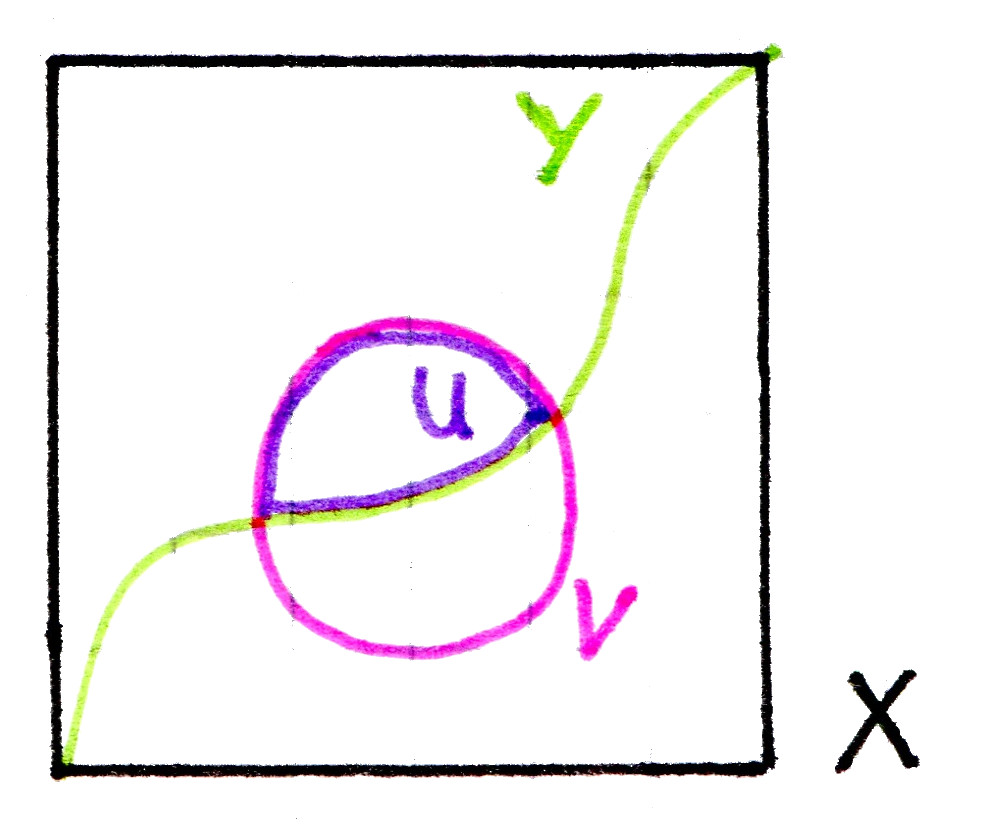
\includegraphics[width=.5\textwidth]{img014-1}
        \caption{Graphische Darstellung der Teilraum-Topologie}
      \end{figure}
    \end{minipage}

    \begin{minipage}{.45\textwidth}
      \item \term{Produkttopologie}\label{def:produkttopologie}: $ (X, \O_X) $ und $ (Y, \O_Y) $ zwei topologische Räume. Eine Teilmenge $ W \subseteq X \times Y $ ist \emph{offen} in der \emph{Produkt-Topologie} $ \Leftrightarrow \ \forall (x, y) \in W \ \exists $ \hyperref[def:umgebung]{Umgebung} $ U $ von $ x $ in $ X $ und $ V $ von $ y $ in $ Y $ sodass das ``Kästchen'' $ U \times V \subseteq W $. \\
      \textbf{Achtung!} Nicht jede offene Menge in $ X \times Y $ ist ein Kästchen: die Vereinigung von zwei Kästchen ist beispielsweise auch offen.
    \end{minipage}
    \hfill
    \begin{minipage}{.45\textwidth}
      \begin{figure}[H]
        \label{img014-3}
        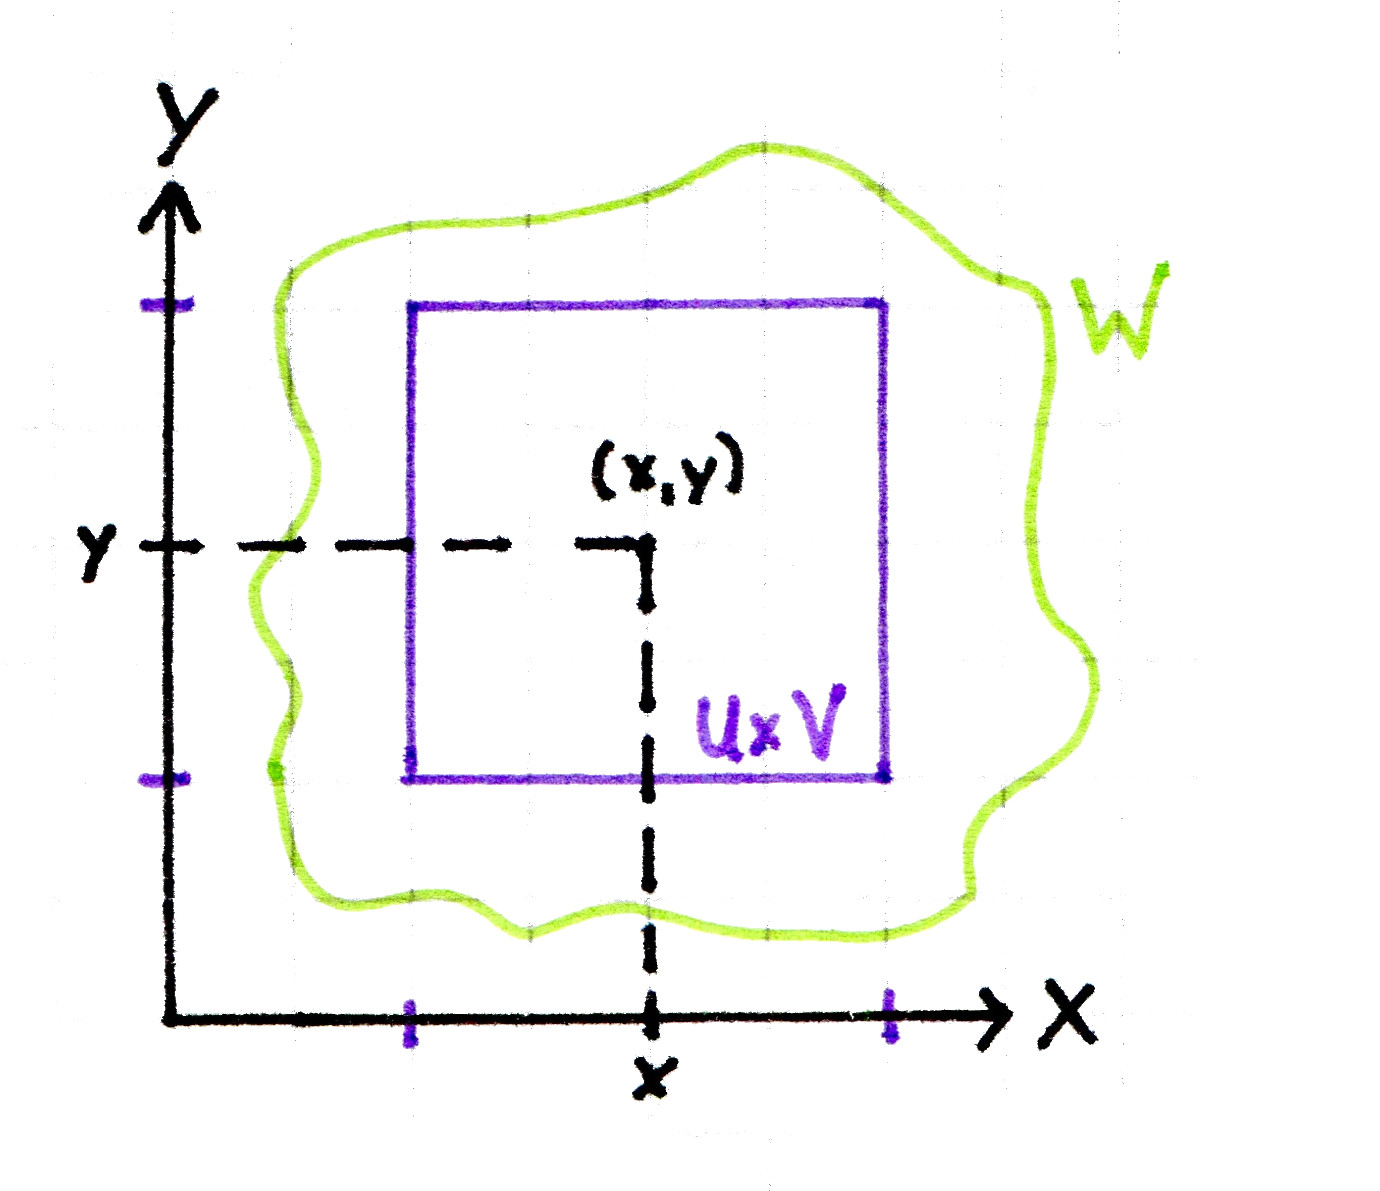
\includegraphics[width=\textwidth]{img014-3}
        \caption{Punkt $ (x,y) $ und sein $ U \times V $-Kästchen}
      \end{figure}
    \end{minipage}
    \textbf{Beispiel}: $ X = \R $ mit Standard-Topologie, dann ist
    \begin{equation*}
      \underbrace{X \times \cdots \times X}_{x \text{ mal}} = \R^n
    \end{equation*}
    induzierter topologischer Raum.

    \item \term{Quotiententopologie}: $ (X, \O) $ topologischer Raum, $ \sim $ Äquivalenzrelation\footnote{Impliziert Partitionierung von $ X $ in disjunkte Teilmengen} auf $ X $. Für $ x \in X $ sei $ [x] \coloneqq  \{ y \in X : y \sim x \} $ die Äquivalenzklasse von $ x $, $ X/\sim $ die Menge der Äquivalenzklassen und
    \begin{align*}
      \pi : X &\to X/\sim \\
      x &\mapsto [x]
    \end{align*}
    die kanonische Projektion (surjektiv!). \\
    Die \emph{Quotienten-Topologie} auf $ X/\sim $ nutzt: \\
    $ U \subset X/\sim $ ist \underline{offen} $ \overset{\text{Def.}}{\Leftrightarrow} \pi^{-1}(U) $ ist offen in $ X $. \\
    \emph{Beispiel}: $ X = \R $ mit \hyperref[bsp:standardtopologie]{Standard-Topologie} (induziert durch \hyperref[bsp:standardmetrik]{Standard-Metrik} $ d_\R(s,t) = \vert s-t \vert $). \\
    Seien $ s, t \in \R $. Wir definieren
    \begin{equation*}
      s \sim t \overset{\text{Def.}}{\Leftrightarrow} \ \exists \ m \in \Z : t = s + 2\pi m\text{.}
    \end{equation*}
    Dann ist
    \begin{equation*}
      \R/\sim \underset{\text{bijektiv}}{=} S' = \text{ Einheitskreis}\text{.}
    \end{equation*}
    Anstatt dies heuristisch auszudrücken kann dies auch explizit getan werden:
    \begin{align*}
      \R &\to S' = \{ z \in \C : \vert z \vert = 1 \} = \{ (x, y) \in \R : x^2+y^2 = 1 \} \\
      t &\mapsto e^{\i t}\text{.}
    \end{align*}
    \begin{figure}[H]
      \label{img015-2}
      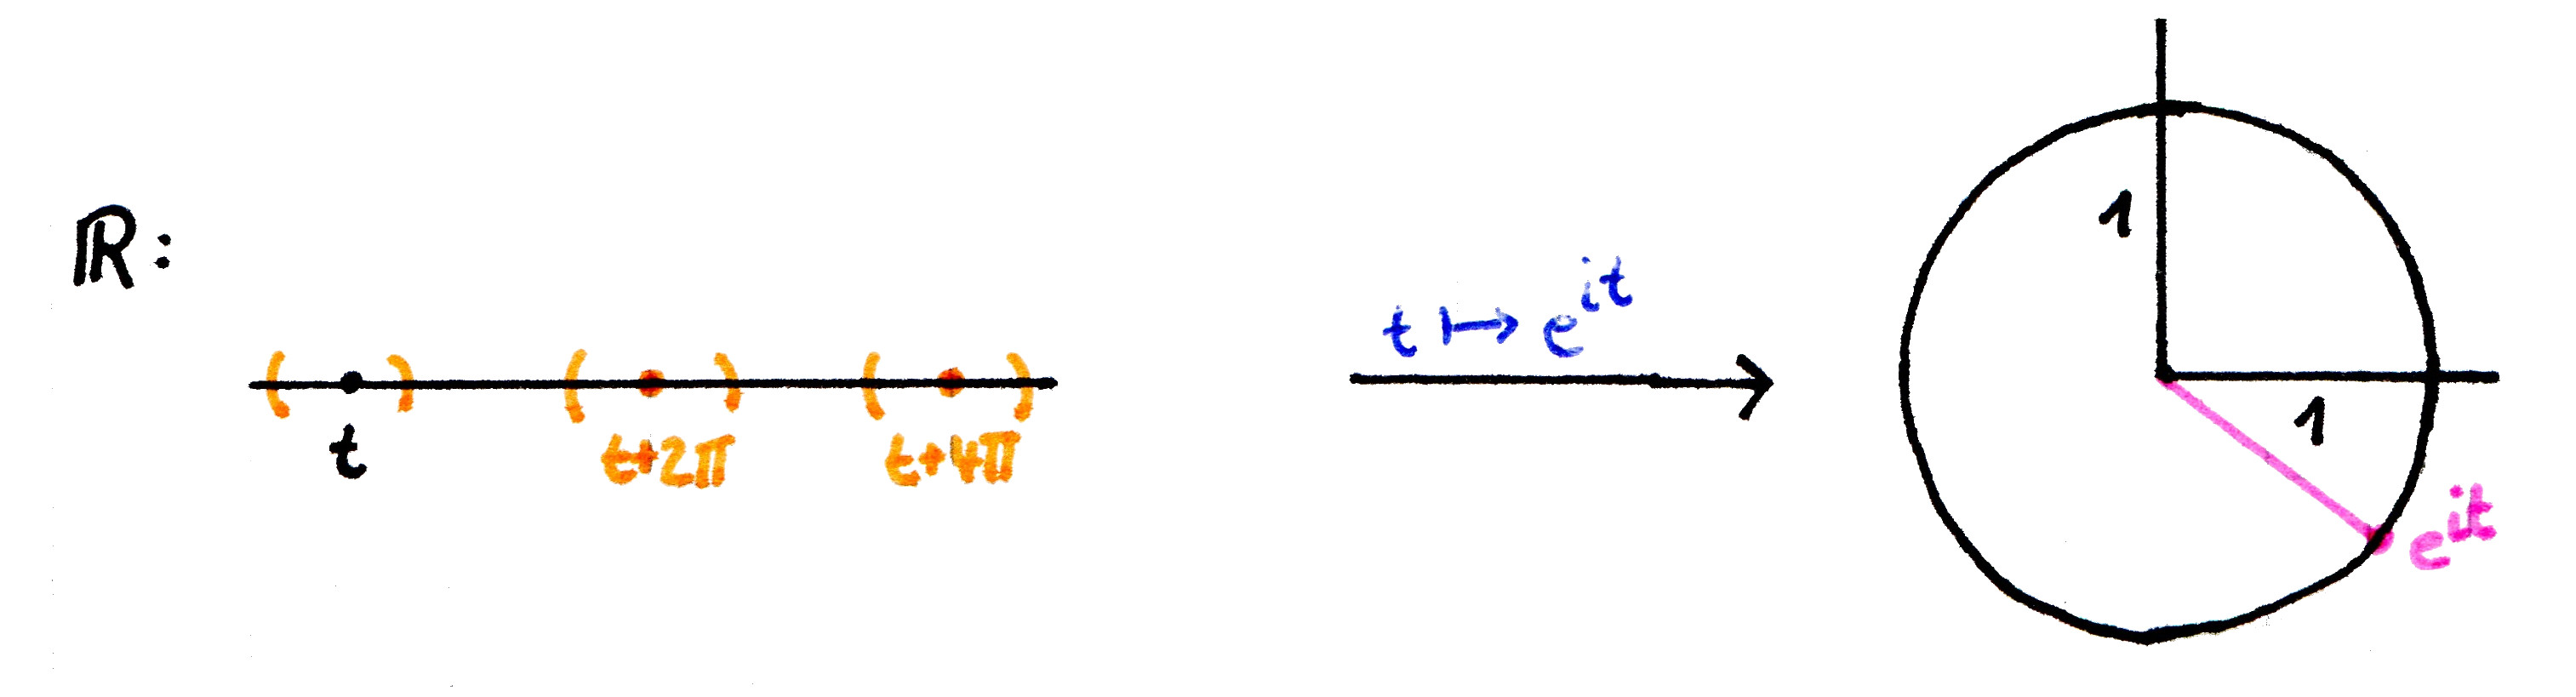
\includegraphics[width=.75\textwidth]{img015-2}
      \caption{Quotiententopologie auf $ \R $}
    \end{figure}
    \emph{Bemerkung}: Andere Interpretation via Gruppen-Aktionen. \\
    $ G = (\Z, +) $ operiert auf $ X = \R $. \\
    \emph{Bahnen-Raum} $ = \R/\sim $ mit
    \begin{align*}
      \Z \times \R &\to \R \\
      (m, t) &\mapsto t + 2\pi m\text{.}
    \end{align*}
    Die Äquivalenzklasse $ [t] $ ist die Bahn von
    \begin{equation*}
      t = \Z*t = \{ t+2\pi m : m \in \Z \}\text{,}
    \end{equation*}
    mehr dazu später.
  \end{enumerate}
\end{remark}

\section{Hausdorffsches Trennungsaxiom}
\begin{remark}[Hausdorffsches Trennungsaxiom $ T_2 $]
  \label{def:hausdorffsch}
  Ein \hyperref[def:topologie]{topologischer Raum} $ (X,\O) $ heißt \term{hausdorffsch}, falls man zu je zwei verschiedenen Punkten $ p,q \in X $ disjunkte \hyperref[def:umgebung]{Umgebungen} finden kann, also Umgebungen $ U \ni p $ und $ V \ni q $ mit $ U \cap V = \varnothing $. \\
  \emph{Beispiel}:
  \begin{enumerate}
    \item \hyperref[def:metrischerRaum]{Metrische Räume} sind \hyperref[def:hausdorffsch]{hausdorffsch}.
    \begin{proof}
       Sei $ d(p,q) \eqqcolon \epsilon $. \\
       Behauptung: $ B_{\epsilon/3}(p) \cap B_{\epsilon/3}(q) = \varnothing $. \\
       Sei $ z $ in $ B_{\epsilon/3}(p) \cap B_{\epsilon/3}(q) $. Dann gilt
       \begin{equation*}
         d(p,q) \overset{\triangle\text{-Ugl.}}{\leq} d(p,z)+d(z,q) \leq \tfrac{\epsilon}{3} + \tfrac{\epsilon}{3} = \tfrac{2\epsilon}{3} < \epsilon \quad \lightning
       \end{equation*}
     \end{proof} 
    \item $ (\R, \hyperref[bsp:standardtopologie]{\O_\text{standard}}) $ ist hausdorffsch, da die Standard-Topologie von der \hyperref[def:metrik]{Metrik} induziert wird.
    \item $ (\R, \hyperref[bsp:zariskitopologie]{\O_\text{Zariski}}) $ ist \underline{nicht} hausdorffsch: offene Mengen sind Komplemente von endlich vielen Punkten, also für $ p, q \in \R, \ p \neq q $:
    \begin{align*}
      U_p &= \R \setminus \{ p_1, \dots, p_n \} \\
      U_q &= \R \setminus \{ q_1, \dots, q_k \}\text{,}
    \end{align*}
    also $ U_p \cap U_q \neq \varnothing $.
  \end{enumerate}
  \emph{Wichtige Konsequenz von ``hausdorffsch''}: In einem Hausdorff-Raum hat jede Folge höchstens einen Limespunkt/Grenzwert.\footnote{\textbf{Erinnerung: Konvergenz}\label{def:konvergenz}: $ (x_n)_{n \in \N} \subset X $ (\hyperref[def:topologie]{top. Raum}). $ X \ni a $ heißt \emph{Limes} um $ (x_n)_{n \in \N} $ falls es zu jeder \hyperref[def:umgebung]{Umgebung} $ U $ von $ a $ ein $ n_0 \in \N $ gibt, sodass $ x_n \in U \ \forall n \geq n_0 $.}
\end{remark}

\begin{remark}[Eigenschaften von Hausdorff-Räumen]
  \
  \begin{enumerate}
    \item Jeder Teilraum (mit \hyperref[def:teilraumtopologie]{Teilraum-Topologie}) eines \hyperref[def:hausdorffsch]{Hausdorff-Raumes} ist hausdorffsch. 
    \item $ X, Y $ Hausdorff-Räume $ \Rightarrow $ $ X \times Y $ ist Hausdorff-Raum bezüglich \hyperref[def:produkttopologie]{Produkt-Topologie}.
  \end{enumerate}
\end{remark}

\section{Stetigkeit}

\begin{definition}[Stetigkeit]
  \label{def:stetig}
  $ (X, \O_X) $, $ (Y, \O_Y) $ \hyperref[def:topologie]{topologische Räume}. Eine Abbildung $ f : X \to Y $ heißt \term{stetig}, falls die Urbilder von offenen Mengen in $ Y $ offen sind in $ X $.
\end{definition}

\begin{example}[Einfache {\hyperref[def:stetig]{Stetigkeiten}}]
  \
  \begin{enumerate}
    \item $ \text{Id}: X \to X $, $ x \mapsto x $ ist stetig.
    \item Die Komposition von stetigen Abbildungen ist stetig.
    \item Für $ (X, \O) = (\R, \hyperref[bsp:standardtopologie]{\O_\text{standard}}) = (Y, \O_Y) $ gibt es unendlich viele Beispiele in Analysis I. \\
    Für \hyperref[def:metrischerRaum]{metrische Räume} ist diese Definition äquivalent zur $ \epsilon $-$ \delta $-Definition und zur Folgenstetigkeit\footnote{Übungsaufgabe!}.
  \end{enumerate}
\end{example}

\begin{definition}[Homöomorphismus]
  \label{def:homoeomorphismus}
  \
  \begin{itemize}
    \item Eine bijektive Abbildung $ f: X \to Y $ zwischen \hyperref[def:topologie]{topologischen Räumen} heißt \term{Homöomorphismus}, falls $ f $ und $ f^{-1} $ \hyperref[def:stetig]{stetig} sind.
    \item $ X $ und $ Y $ heißen \term{homöomorph}, falls ein Homöomorphismus $ f: X \to Y $ existiert (notiere $ X \cong Y $). 
  \end{itemize}
\end{definition}

\begin{remark}[Homöomorphismengruppe]
  \
  \begin{itemize}
    \item $ \text{Id}_X: X \to X $, $ x \mapsto x $ ist \hyperref[def:homoeomorphismus]{Homöomorphismus}.
    \item Verkettungen von Homöomorphismen sind wieder Homöomorphismen.
    \item Inverses eines Homöomorphismus ist ein Homöomorphismus.
  \end{itemize}
  Aus diesen drei Punkten folgt, dass die Homöomorphismen eine Gruppe bilden.
\end{remark}

\begin{example}[Einfache {\hyperref[def:homoeomorphismus]{Homöomorphismen}}]
  \
  \begin{itemize}
    \item $ [0,1] = \{ t \in \R : 0 \leq t \leq 1 \} \cong [a,b] $ mit $ a < b \in \R $ \\ (via $ f(t) = a+t(b-a) $).
    \item $ (0,1) = \{ t \in \R : 0 < t < 1 \} \cong (a,b) $ mit $ a < b $ beliebig. 
    \item $ \R \cong (-1, 1) \cong (0,1) $ \\ (z.B. via $ t \mapsto \tanh t = \tfrac{e^{2t}-1}{e^{2t}+1} $).
    \item \hyperref[def:stetig]{Stetig} und injektiv, aber \underline{kein} Homöomorphismus! \\
      $ f: [0,1) \to S^1 $, $ t \mapsto e^{2\pi\i t} = \cos(2\pi t) + \i\sin(2\pi t) $ ist stetig, injektiv, aber kein Homöomorphismus.
    \item Projektions-Abbildungen sind stetig, z.B. $ p_1: X_1 \times X_2 \to X_1 $, $ (x_1,x_2) \mapsto x_1 $: Für $ U $ offen in $ X_1 $ ist $ p^{-1}(U) = U \times X_2 $ offen bezüglich der \hyperref[def:produkttopologie]{Produkttopologie}.
    \item \hyperref[def:metrischerRaum]{Metrische Räume} $ (X, d_X) $, $ (Y, d_Y) $ und \hyperref[def:isometrie]{Isometrie} $ f: X \to Y $, also eine bijektive Abbildung, so dass
      \begin{equation*}
        \forall x, y \in X : d_Y(f(x), f(y)) = d_X(x, y)\text{.}
      \end{equation*}
      \emph{Behauptung}: $ f $ ist Homöomorphismus (bzgl. der durch \hyperref[def:metrik]{Metrik} definierten \hyperref[def:topologie]{Topologien}).
      \begin{proof}
        (über $ \epsilon $-$ \delta $-Definition): $ \delta \coloneqq \epsilon $. \\
        $ d_X(x, y) < \delta \Rightarrow d_Y(f(x), f(y)) = d_X(x,y) < \delta = \epsilon $, also ist $ f $ stetig. \\
        Analog für $ f^{-1} $.
      \end{proof}
    \item $ S^n = \{ x \in R^{n+1} : \Vert x \Vert^2 = 1 \} $ ist die $ n $-dimensionale \hyperref[bsp:einheitssphaere]{Einheitssphäre} in $ \R^{n+1} $. \\
      $ e_{n+1} = (0,\dots,0,1) $ sei der ``Nordpol'' von $ S_n $. \\
      \emph{Behauptung}: $ S^n\setminus\{ e_{n+1} \} \cong \R^n $.
      \begin{proof}
        (via stereographische Projektion):
        \begin{equation*}
          \R^n \cong \{ x \in \R^{n+1} : x_{n+1} = 0 \}\text{,}
        \end{equation*}
        \begin{equation*}
          f(x) \coloneqq (\tfrac{x_1}{1-x_{n+1}}, \dots, \tfrac{x_n}{1-x_{n+1}}) \text{ stetig,}
        \end{equation*}
        \begin{equation*}
          f^{-1}: \R^n \to S^n\text{,} \quad y \mapsto \left( \tfrac{2y_1}{\Vert y \Vert^2+1}, \dots, \tfrac{2y_n}{\Vert y \Vert^2+1}, \tfrac{\Vert y \Vert^2-1}{\Vert y \Vert^2+1} \right)\text{ auch stetig.}
        \end{equation*}
        Also ist $ f $ homöomorph.
      \end{proof}
      \emph{Achtung}: $ S^n $ ist \underline{nicht} homöomorph zu $ \R^n $ (da $ S^n $ \hyperref[def:kompakt]{kompakt} und $ \R^n $ nicht kompakt ist, mehr dazu später).
      \begin{figure}[H]
        \label{img018-2}
        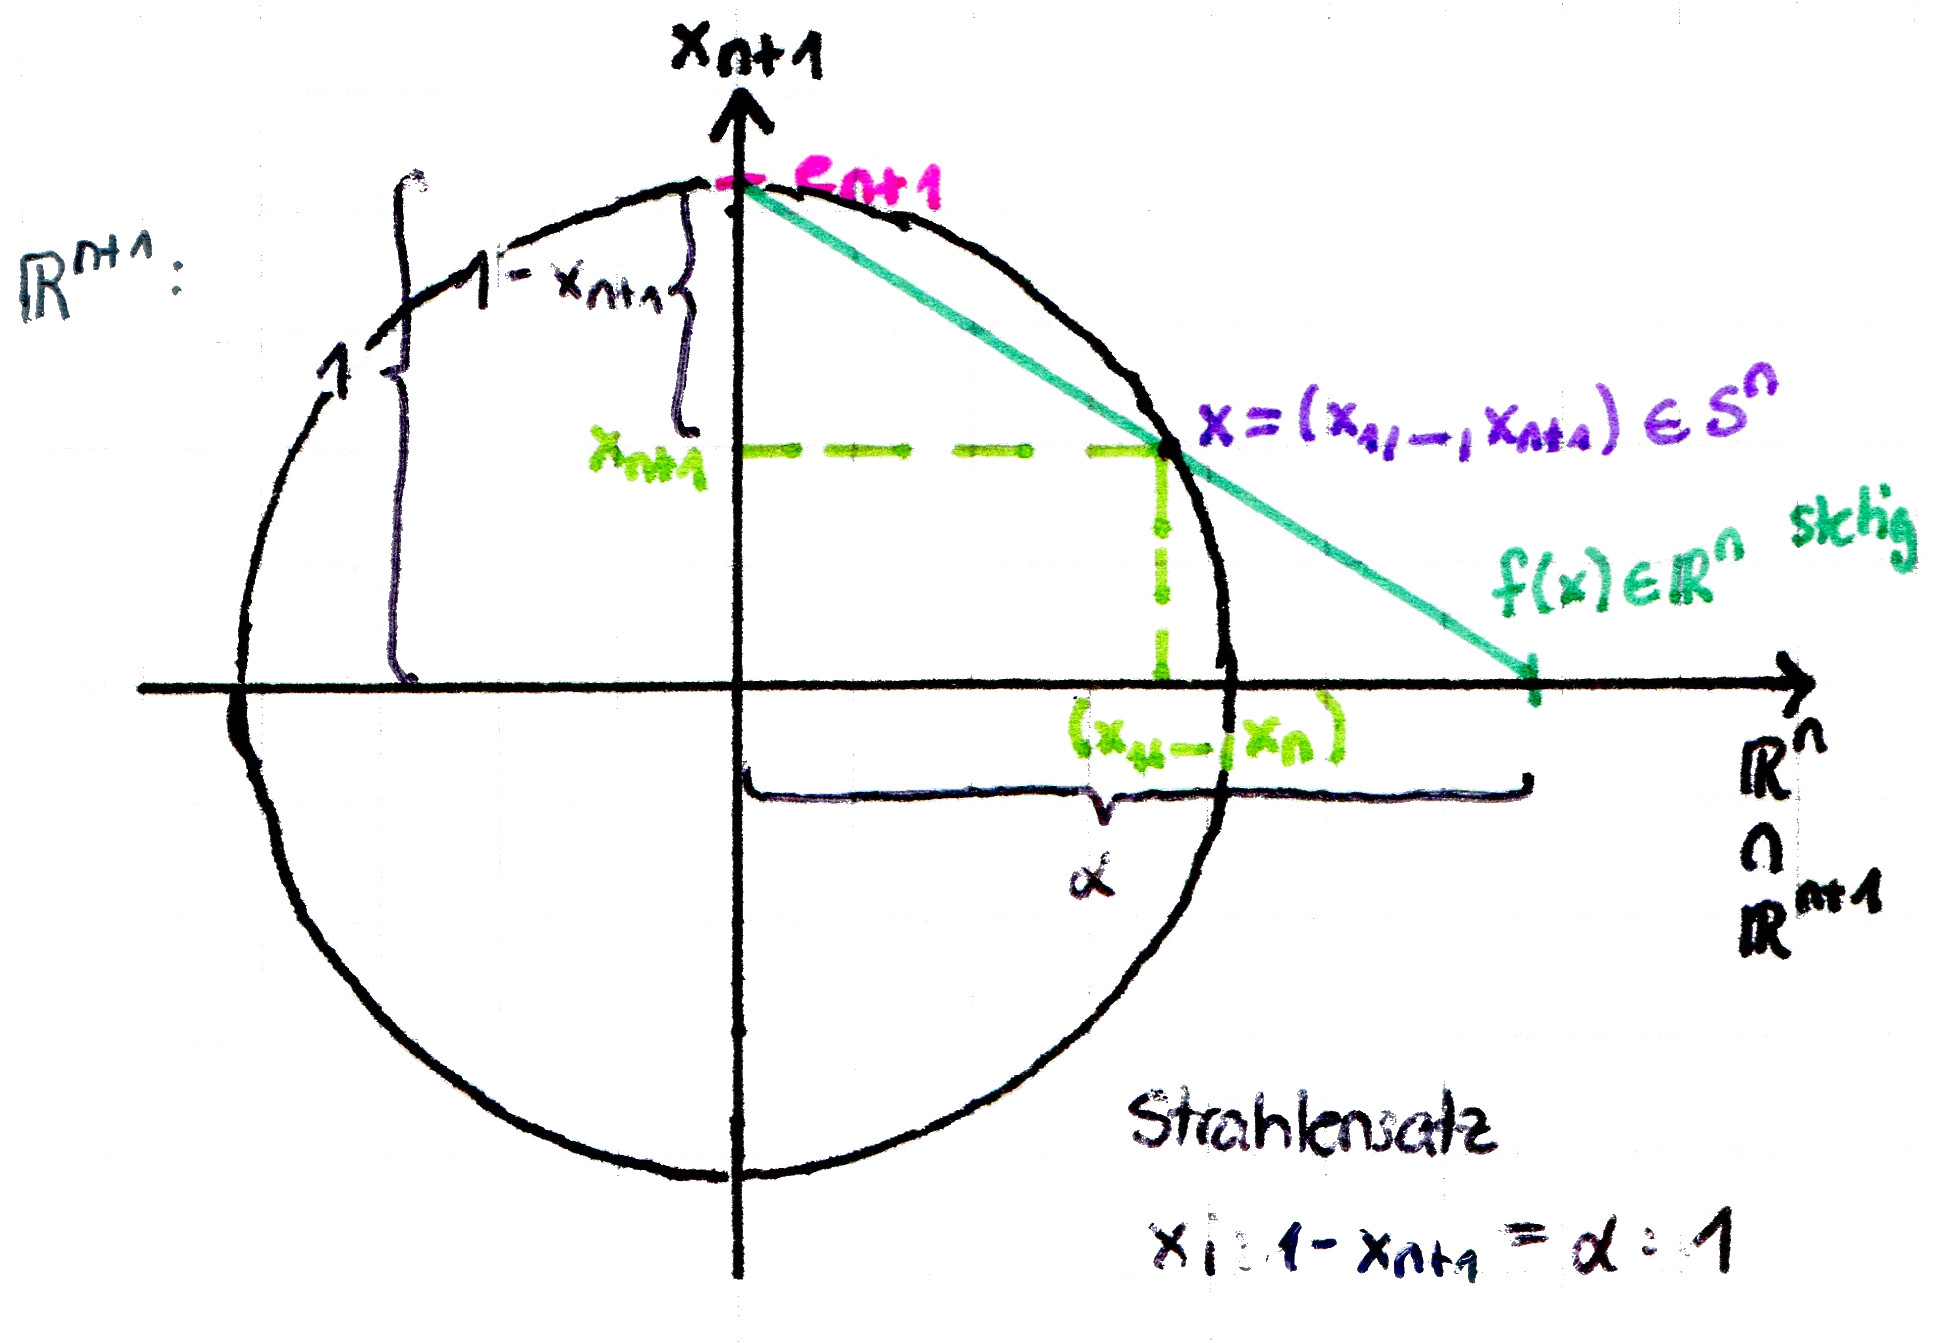
\includegraphics[width=.5\textwidth]{img018-2}
        \caption{Stereographische Projektion}
      \end{figure}
  \end{itemize}
\end{example}

\begin{remark}[{\hyperref[def:isometrie]{Isometrien}}-Untergruppe]
  Isometrien bilden eine Untergruppe der \hyperref[def:homoeomorphismus]{Homöomorphismen} von $ X $ (versehen mit von der \hyperref[def:metrik]{Metrik} induzierten Topologie):
  \begin{equation*}
    \text{Isom}(X, d) \subseteq \text{Homö}(X, \O_d) \subseteq \text{Bij}(X)\text{.}
  \end{equation*}
\end{remark}

\begin{remark}[Exkurs 1: Kurven]
  \label{exkurs:kurve}
  \ \\
  \begin{minipage}{.45\textwidth}
    \vspace{0.1cm}
    Was ist eine Kurve? \\
    \emph{Naive Definition}: Eine Kurve ist ein stetiges Bild eines Intervalls. \\
    \emph{Problem}: $ \exists $ stetige, surjektive (aber nicht injektive) Abbildungen $ I = [0,1] \to I^2 $ (``Peano-Kurven'', ``space-filling curves'')\footnotemark.
    \vspace{0.1cm}
  \end{minipage}
  \footnotetext{Mehr dazu in Königsberger --- Analysis I.}
  \hfill
  \begin{minipage}{.45\textwidth}
    \vspace{0.1cm}  
    \begin{figure}[H]
      \label{img019-1}
      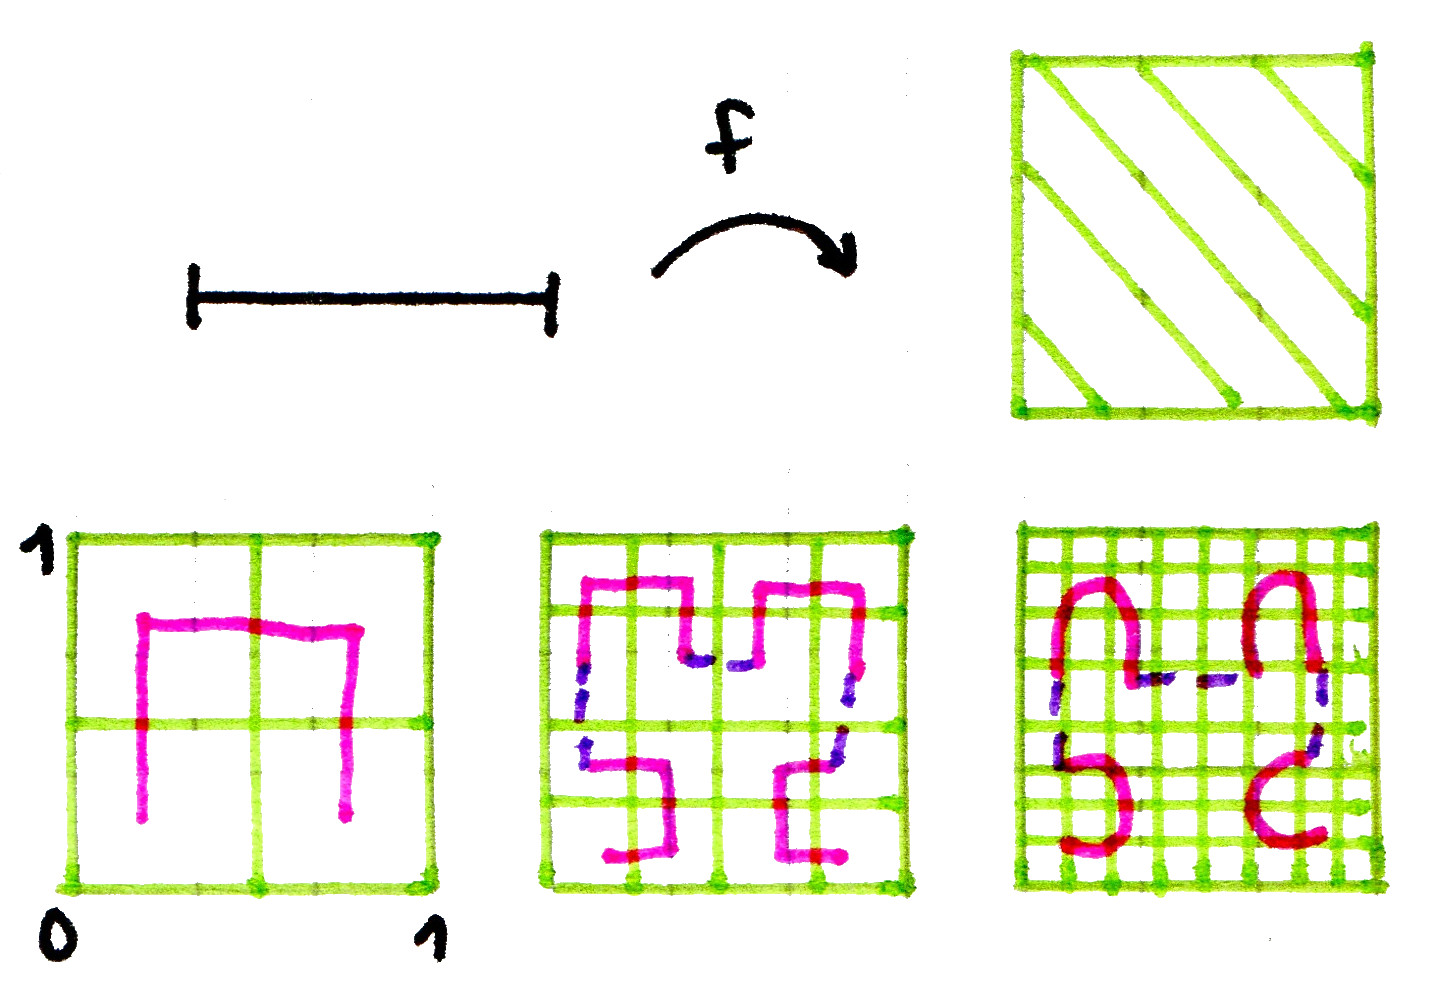
\includegraphics[width=.8\textwidth]{img019-1}
      \caption{Space-filling curves}
    \end{figure}
    \vspace{0.1cm}
  \end{minipage}
  \emph{Ausweg 1}: \emph{Jordan-Kuven} (bzw. geschlossene J-Kurven). \\
    $ \coloneqq $ top. Raum, \hyperref[def:homoeomorphismus]{homöomorph} zu $ I = [0,1] $ (J-Kurve) \\
    $ \coloneqq $ top. Raum, homöomorph zu $ S^1 $ (geschlossene J-Kurve) \\
  \emph{Ausweg 2}: \emph{reguläre stetig differenzierbare Kurven} (lokal injektiv). \\
  \emph{Verwendung}: z.B. \emph{Knoten} --- spezielle geschlossene Jordankurve als Unterraum von $ \R^3 $:
  \begin{equation*}
    \exists \ f : S^1 \to \R^3 \text{ mit } f(S^1) \cong S^1
  \end{equation*}
  mit \hyperref[def:teilraumtopologie]{Teilraumtopologie} von $ R^3 $. \\
  Zwei Knoten $ K_1 $, $ K_2 \subset \R^3 $ sind \emph{äquivalent}, falls es einen Homöomorphismus $ h $ von $ \R^3 $ gibt mit $ h(K_1) = K_2 $.\footnote{\textbf{Knotentheorie} studiert die Äquivalenz von Knoten, siehe z.B. Sossinsky --- Mathematik der Knoten}
  \begin{figure}[H]
    \label{img019-4}
    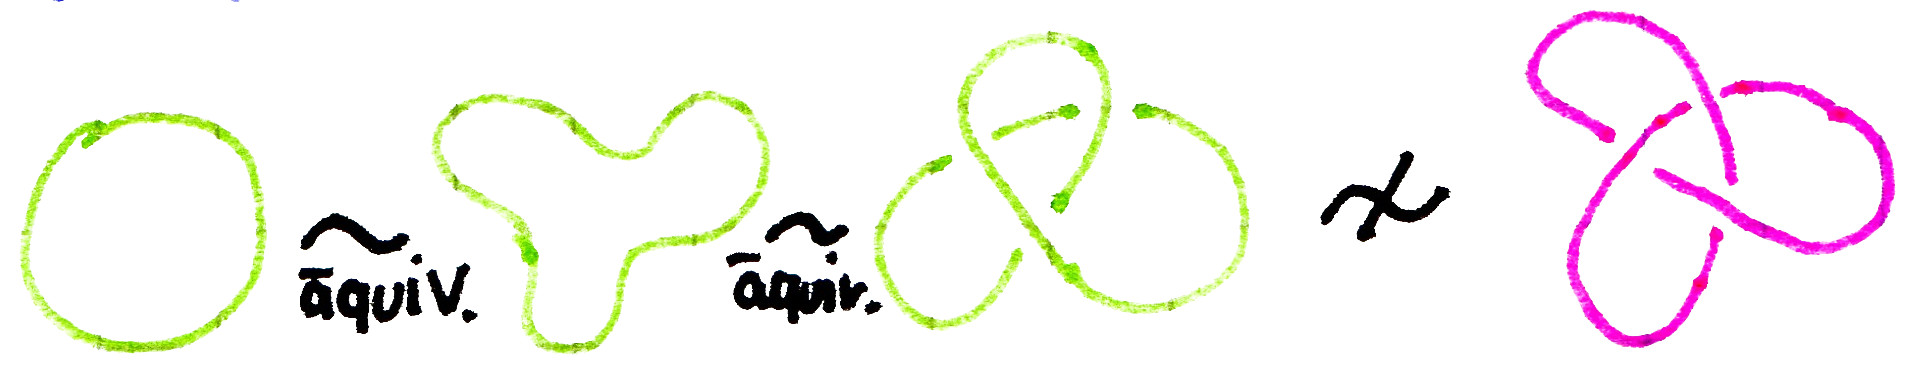
\includegraphics[width=.5\textwidth]{img019-4}
    \caption{Äquivalente und nicht-äquivalente Knoten}
  \end{figure}
\end{remark}

\begin{remark}[Exkurs 2: Topologische Gruppen]
  \label{exkurs:topologischeGruppe}
  Eine \term{topologische Gruppe} ist eine Gruppe versehen mit einer \hyperref[def:topologie]{Topologie}, sodass die Gruppenmultiplikation
  \begin{equation*}
    m: G \times G \to G, \quad (g,h) \mapsto g*h
  \end{equation*}
  mit \hyperref[def:produkttopologie]{Produkt-Topologie} und die Inversenbildung
  \begin{equation*}
    i: G \to G, \quad g \mapsto g^{-1 }
  \end{equation*}
  \hyperref[def:stetig]{stetig} sind.
\end{remark}

\begin{example}[Topologische Gruppen]
  \
  \begin{enumerate}
    \item $ G $ beliebige Gruppe mit \hyperref[bsp:diskreteTopologie]{diskreter Topologie} ist \hyperref[exkurs:topologischeGruppe]{topologische Gruppe}.
    \item $ \R^n $ mit \hyperref[bsp:standardtopologie]{Standard-Topologie} ist abelsche topologische Gruppe.
    \item $ \R \setminus \{ 0 \} $, $ \C \setminus \{ 0 \} $ sind multiplikative topologische Gruppen.
    \item $ H \subset G $ Untergruppe einer topologischen Gruppe ist topologische Gruppe bzgl. \hyperref[def:teilraumtopologie]{Teilraumtopologie}.
    \item Das Produkt von topologischen Gruppen mit \hyperref[def:produkttopologie]{Produkttopologie} ist eine topologische Gruppe.
    \item $ \text{GL}(n,\R) = \{ A \in \underbrace{\R^{n \times n}}_{= \R^{n^2}} : \det A \neq 0 \} $ allg. reelle lineare Gruppe. \\
      $ \text{GL}(n,\R) \subset \R^{n^2} $ versehen mit \hyperref[def:teilraumtopologie]{Teilraum-Topologie} induziert von $ \R^{n^2} = \R^{n \times n} $ ist topologische Gruppe:
      \begin{itemize}
        \item Matrizenmultiplikation ist \hyperref[def:stetig]{stetige} Abbildung ($ \R^{n^2} \times \R^{n^2} \to \R^{n^2} $),
        \item Inversen-Abbildung ist ebenfalls stetig (wegen expliziter Formel für $ A^{-1} $).
      \end{itemize}
    \item $ \text{SO}(n) = \{ A \in \text{GL}(n,\R) : A^\top A = E_n, \det A = 1 \} $ ist die \term{spezielle orthogonale Gruppe}. Sie ist eine topologische Gruppe nach Beispiel 4 und 6. \\
      Insbesondere ist
      \begin{equation*}
        \text{SO}(2) = \left\{ \begin{pmatrix}
          \cos \theta & -\sin \theta \\
          \sin \theta & \cos \theta
        \end{pmatrix} : \theta \in [0, 2\pi] \right\} \cong S'
      \end{equation*}
      eine abelsche topologische Gruppe.
  \end{enumerate}
\end{example}

\section{Zusammenhang}

\begin{definition}[Zusammenhängend]
  \label{def:zusammenhaengend}
  Ein \hyperref[def:topologie]{topologischer Raum} $ (X, \O) $ heißt \term{zusammenhängend}, falls $ \varnothing $ und $ X $ die einzigen gleichzeitig offenen und abgeschlossenenen Teilmengen von $ X $ sind. \\
  \textbf{Äquivalent}: $ X $ ist zusammenhängend $ \Leftrightarrow X $ ist \emph{nicht} disjunkte Vereinigung von 2 offenen, nichtleeren Teilmengen.
  \begin{proof}
    $ A \subset X $ offen und abgeschlossen $ \Leftrightarrow A $ und $ X \setminus A $ offen $ \Leftrightarrow A $ und $ X \setminus A $ abgeschlossen.
  \end{proof}
\end{definition}

\begin{example}[Zusammenhang]
  \
  \begin{enumerate}
    \item $ \R $ (und ebenso beliebige Intervalle) ist \hyperref[def:zusammenhaengend]{zusammenhängend}, $ \R \setminus \{ 0 \} $ ist \emph{nicht} zusammenhängend.
    \begin{proof}
      Sei $ I \subseteq \R $ (abgeschlossenes oder offenes oder halboffenes) Intervall. \\
      \emph{Annahme}: $ I \neq U \neq \varnothing $, sei eine offen-abgeschlossene Teilmenge von $ I $. Dann gibt es mindestens einen Punkt $ u \in U $ und $ v \in I \setminus U $. OBdA $ u < v $. Setze $ U_0 \coloneqq \{ x \in U : x < v \} $ und $ c \coloneqq \sup U_0 $. Also $ u \leq c \leq v $. Weiter ist $ c \in U $, da $ U $ abgeschlossen ist. Eine ganze \hyperref[def:umgebung]{Umgebung} von $ c $ gehört auch zu $ U $, da $ U $ offen ist. Damit gehört eine ganze Umgebung von $ c $ auch zu $ U_0 \quad \lightning $
    \end{proof}
  \end{enumerate}
\end{example}

\begin{remark}[Ergänzung: Zusammenhang von Teilmengen]
  \emph{Allgemein}: Eine Teilmenge $ B \subset X $ heißt \term{zusammenhängend}, falls sie bezüglich der \hyperref[def:teilraumtopologie]{Teilraumtopologie} zusammenhängend ist.
\end{remark}

\begin{remark}[Einpunktige Mengen]
  Einpunktige Mengen sind \hyperref[def:zusammenhaengend]{zusammenhängend}: $ \{ x \} $ mit \hyperref[def:teilraumtopologie]{Teilraumtopologie} ist diskret (also sind $ \{ x \} $ und $ \varnothing $ die einzigen offenen Mengen).
\end{remark}

\begin{definition}[Zusammenhangskomponente]
  \label{def:zusammenhangskomponente}
  Sei $ x \in X $. Die \term{Zusammenhangskomponente} $ Z(x) $ ist die Vereinigung aller \hyperref[def:zusammenhaengend]{zusammenhängenden} Teilmengen, die $ x $ enthalten.
\end{definition}

\begin{lemma}[Eigenschaften {\hyperref[def:zusammenhaengend]{zusammenhängender}} Mengen]
  \
  \begin{enumerate}
    \item $ A $ ist zusammenhängend $ \Rightarrow \overline{A} $ (abgeschlossene Hülle von $ A $) ist zusammenhängend.
    \item $ A $, $ B $ zusammenhängend, $ A \cap B \neq \varnothing \Rightarrow A \cup B $ zusammenhängend.\footnote{Übungsaufgabe, es wird nur die Definition von Zusammenhang benötigt.} 
  \end{enumerate}
\end{lemma}

\begin{remark}[Zusammenhängende Mengen bilden disjunkte Zerlegung]
  \ \\ \hyperref[def:zusammenhangskomponente]{Zusammenhangskomponenten} von $ X $ sind zusammenhängende Mengen und bilden eine disjunkte Zerlegung von $ X $.
  \begin{proof}
    Definiere eine Äquivalenzrelation (für $ x, y \in X $):
    \begin{equation*}
      x \sim y \overset{\text{Def}}{\Leftrightarrow} \exists \text{ zusammenhängende Menge } A : x, y \in A\text{.}
    \end{equation*}
    $ \sim $ ist Äquivalenzrelation:
    \begin{itemize}
      \item \textbf{Reflexivität}: $ x \sim x $, denn die einpunktige Menge $ \{ x \} $ ist zusammenhängend. 
      \item \textbf{Symmetrie}: $ x \sim y \Rightarrow y \sim x $ nach Definition.
      \item \textbf{Transitivität}: $ x \sim y \wedge y \sim z \Rightarrow x \sim z $: \\
        $ x \sim y: \exists \ A $ zusammenhängend mit $ x,y \in A $. \\
        $ y \sim z: \exists \ B $ zusammenhängend mit $ y,z \in B $. \\
        Also $ y \in A \cap B \overset{\text{Lemma}}{\Rightarrow} A \cup B $ zusammenhängend.
    \end{itemize}
  \end{proof}
\end{remark}

\begin{example}[{{\hyperref[def:zusammenhangskomponente]{Zusammenhangskomponenten}}}]
  \
  \begin{enumerate}
    \item $ \R \setminus \{ t \} = \{ s \in \R : s < t \} \cup \{ s \in \R : s > t \} $ hat 2 Zusammenhangskomponenten.
    \item $ \mathbb{Q} = \R \setminus \{ \text{irrationale Zahlen} \} $ mit \hyperref[def:teilraumtopologie]{Teilraum-Topologie} von $ (\R, \O_\text{standard}) $ ist \term{total unzusammenhängend}, d.h. alle Zusammenhangskomponenten sind einpunktig. \\
    \begin{proof}
      \emph{Annahme}: $ A \subset \mathbb{Q} $ mit mindestens $ 2 $ verschiedenen Punkten. \\
      \emph{Behauptung}: $ A $ ist nicht zusammenhängend. \\
      Sei $ \{ q_1, q_2 \} = A \subset \mathbb{Q} $ mit $ q_1 \neq q_2 $ (oBdA $ q_1 < q_2 $). Sei $ s \in \R \setminus \mathbb{Q} $ mit $ q_1 < s < q_2 $, $ O_1 = \{ t \in \R: t < s \} $, $ O_2 = \{ t \in \R : t > s \} $, $ \widetilde{O_1} = O_1 \cap A $, $ \widetilde{O_2} = O_2 \cap A $. $ \widetilde{O_1} $ und $ \widetilde{O_2} $ sind offen in $ A $ oder in $ \mathbb{Q} $ bezüglich der Teilraumtopoogie. Es ist $ A = \widetilde{O_1} \cup \widetilde{O_2} $ mit $ \widetilde{O_1} \cap \widetilde{O_2} \neq \varnothing $, d.h. $ A $ ist \emph{nicht} zusammenhängend.
    \end{proof}
  \end{enumerate}
\end{example}

\begin{definition}[Weg-Zusammenhängend]
  \label{def:wegzusammenhaengend}
  Sei $ (X, \O) $ ein \hyperref[def:topologie]{topologischer Raum}. $ X $ heißt \term{weg-zusammenhängend}, wenn es zu je zwei Punkten $ p, q \in X $ einen Weg (d.h. stetige Abbildung $ \alpha : [0,1] \to X $ mit $ \alpha(0) = p $ und $ \alpha(1) = q $) zwischen $ p $ und $ q $ gibt.
  \begin{figure}[H]
    \label{img023-2}
    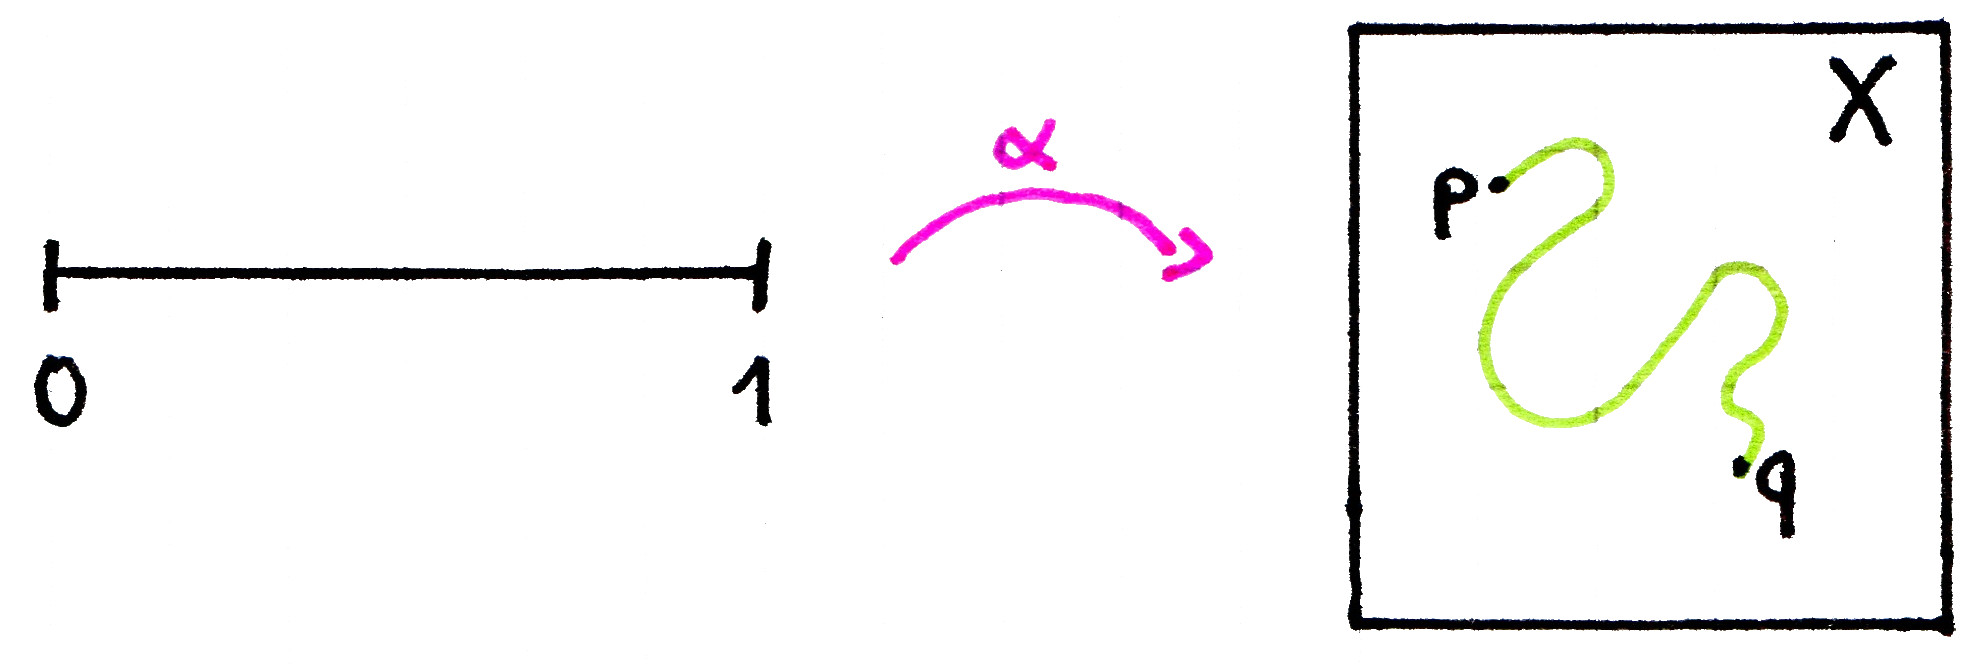
\includegraphics[width=.5\textwidth]{img023-2}
    \caption{Darstellung der Funktionsweise einer solchen Funktion $ \alpha $}
  \end{figure}
\end{definition}

\begin{lemma}[Weg-Zusammenhang]
  $ X $ ist \hyperref[def:wegzusammenhaengend]{weg-zusammenhängend} $ \Rightarrow $ $ X $ ist \hyperref[def:zusammenhaengend]{zusammenhängend}.
  \begin{proof}
    Wäre $ X $ \emph{nicht} zusammenhängend, dann $ \exists $ eine disjunkte Zerlegung $ X = A \cup B $ mit $ A $, $ B $ offen und nicht-leer, $ A \cap B = \varnothing $ mit $ p \in A $ und $ q \in B $. Sei $ \alpha: [0,1] \to X $ ein (stetiger) Weg zwischen $ p $ und $ q $, also $ \alpha(0) = p $ und $ \alpha(1) = q $. Daraus folgt, dass $ [0,1] = \alpha^{-1}(\alpha([0,1])) = \alpha^{-1}(A \cap \alpha([0,1])) \cup \alpha^{-1}(B \cap \alpha([0,1])) \Rightarrow [0,1] \text{ ist nicht zusammenhängend} \quad \lightning $
  \end{proof}

  \begin{minipage}{.45\textwidth}
    \textbf{Achtung}: Umkehrung gilt nicht! Z.B. ``topologische Sinuskurve''\footnotemark $ X $ ist zusammenhängend, aber \emph{nicht} weg-zusammenhängend:
  \end{minipage}
  \footnotetext{\textbf{Details}: Singer-Thorpe p.52}
  \hfill
  \begin{minipage}{.45\textwidth}
    \begin{figure}[H]
      \label{img023-3}
      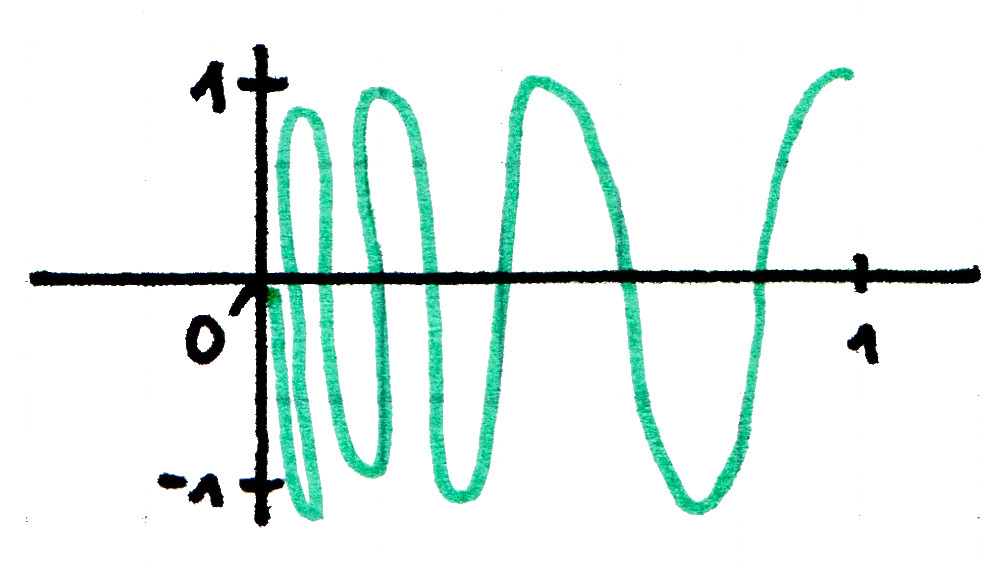
\includegraphics[width=.8\textwidth]{img023-3}
      \caption{Darstellung der ``topologischen Sinuskurve''}
    \end{figure}
  \end{minipage}
  \begin{equation*}
    X \coloneqq \left\{ \left( x, \sin\tfrac{1}{x} \right) \in \R^2 : 0 < x \leq 1 \right\} \cup \{ (0,y) : \vert y \vert < 1 \}\text{.}
  \end{equation*}
\end{lemma}

\begin{lemma}[Weg-Zusammenhang von Bildern]
  \hyperref[def:stetig]{Stetige} Bilder von \\ (\hyperref[def:wegzusammenhaengend]{weg}-)\hyperref[def:zusammenhaengend]{zusammenhängenden} Räumen sind (weg-)zusammenhängend.
  \begin{proof}
    \
    \begin{enumerate}
      \item Sei $ f: X \to X $ stetig und $ f(X) = A \cup B $ eine disjunkte Zerlegung in nichtleere offene Mengen. \\
        Dann ist $ X = f^{-1}(A) \cup f^{-1}(B) $ eine disjunkte Zerlegung.
      \item Seien $ x = f(p) $, $ y = f(q) $ zwei Punkte in $ f(X) $. Es ist $ p = f^{-1}(x) $, $ q = f^{-1}(y) $. \\
        Dann existiert $ a: [0,1] \to X $ mit $ a(0) = p $ und $ a(1) = q $ und somit ist $ f \circ a: [0,1] \to f(X) $ ein \hyperref[def:wegzusammenhaengend]{stetiger Weg} in $ f(X) $. 
    \end{enumerate}
  \end{proof}
\end{lemma}

\begin{corollary}[Zwischenwertsatz]
  Eine \hyperref[def:stetig]{stetige Funktion} $ f: [a,b] \to \R $ nimmt jeden Wert zwischen $ f(a) $ und $ f(b) $ an.
\end{corollary}

\begin{remark}[Test auf {\hyperref[def:homoeomorphismus]{Homöomorphie}} via {\hyperref[def:zusammenhaengend]{Zusammenhang}}]
  \ \\ \emph{Beispiel}: $ \R \cong \R^n $ nur falls $ n = 1 $.
  \begin{proof}
    Wir nehmen an, dass $ R \cong \R^n $ für $ n \geq 1 $. Es ist
    \begin{equation*}
      \underbrace{\R \setminus \{ \text{Punkt} \}}_{\text{nicht zusammenhängend}} \cong \underbrace{\R^n \setminus \{ \text{Punkt} \} }_{\text{zusammenhängend für } n \geq 2} \quad \lightning
    \end{equation*}
    Ebenso: $ [0,1] \cong [0,1]^n $ nur für $ n = 1 $.
  \end{proof}
\end{remark}

\begin{theorem}[von Brouwer]
  $ \R^n \not \cong \R^m $ für $ m \neq n $.
  \begin{proof}
    Der Beweis benutzt den \term{Satz von Gebietstreue}\label{th:satzGebietstreue} (Brouwer):
    \begin{quote}
      \emph{Ist $ U \subseteq $ offen und $ f: U \to \R^n $ eine injektive \hyperref[def:stetig]{stetige} Abbildung, so ist $ f(U) \subseteq \R^n $ offen.}
    \end{quote}
    \emph{Beweisidee}: Ist $ m < n $, so ist
    \begin{equation*}
      j: \R^m \to \R^n, \quad (x_1, \dots, x_m) \mapsto (x_1, \dots, x_m, 0, \dots, 0)
    \end{equation*}
    eine Einbettung und eine injektive, stetige Abbildung von $ \R^m $ auf eine \emph{nicht} offene Teilmenge von $ \R^n $. Wäre $ \R^m \cong \R^n $, so hat man einen Widerspruch zum Satz von Gebietstreue.\footnote{siehe auch Alexandrov-Hopf, Topologie, 1935, Kap. X.2}
  \end{proof}
\end{theorem}

\section{Kompaktheit}

\begin{definition}[(Lokal) kompakt]
  \label{def:kompakt}
  Ein \hyperref[def:topologie]{topologischer Raum} heißt \term{kompakt}, wenn jede offene Überdeckung von $ X $ eine \emph{endliche} Teilüberdeckung besitzt, also
  \begin{align*}
    X &= \bigcup_{i \in I} U_i, \ U_i \text{ offen } \Rightarrow \ \exists \ i_1, \dots, i_k \in I : \\
    X &= U_{i_1} \cup \cdots \cup U_{i_k}
  \end{align*}
  \begin{itemize}
    \item $ A \subseteq X $ heißt \emph{kompakt}, wenn $ A $ bezüglich der \hyperref[def:teilraumtopologie]{Teilraumtopologie} kompakt ist.
    \item $ X $ heißt \emph{lokal kompakt}, wenn jeder Punkt von $ X $ eine kompakte Umgebung besitzt.
  \end{itemize}
\end{definition}

\begin{remark}[Verwendung {\hyperref[def:kompakt]{kompakter Räume}}]
  Kompakte Räume sind oft ``einfacher'' als nicht-kompakte, weil man beispielsweise von lokalen Eigenschaften auf globale schließen kann. \\
  \emph{Begründung}: $ \forall x \in X \ \exists \ U_x : f\vert_{U_x} \leq c_x $. Schreibe $ X = \bigcup_{x \in X}U_x $. Da $ X $ kompakt ist existieren $ x_1, \dots, x_k \in X $, sodass $ X = \bigcup_{i=1}^k U_{x_i} $. \\
  $ \Rightarrow f(x) \leq \text{max}\{ c_{x_1}, \dots, c_{x_k} \} $.
  \begin{figure}[H]
    \label{img025-1}
    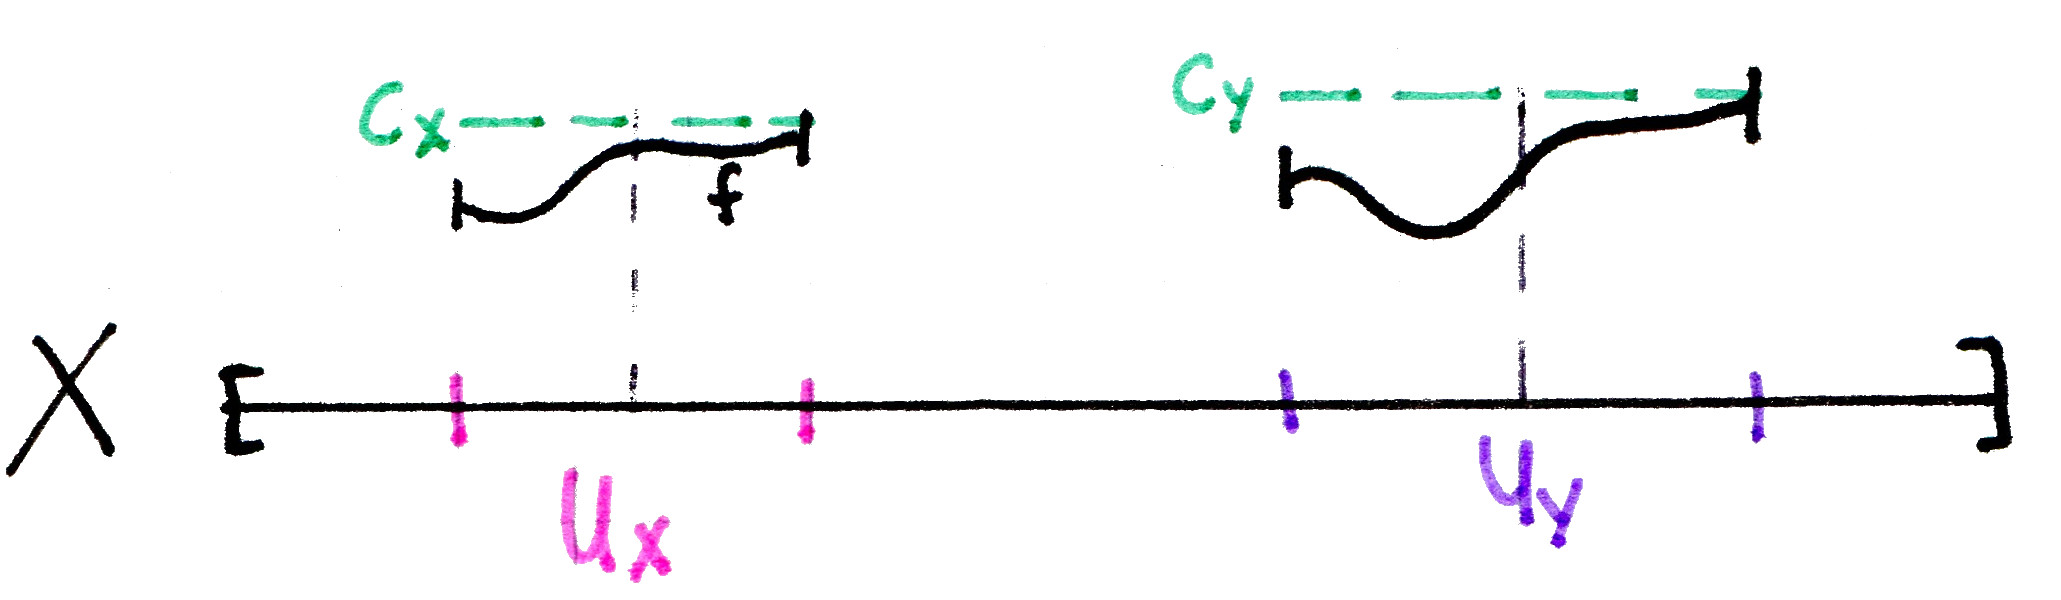
\includegraphics[width=.5\textwidth]{img025-1}
    \caption{Konstruktion zum Schließen von lokalen auf globale Eigenschaften bei kompakten Räumen}
  \end{figure}
\end{remark}

\begin{example}[Beschränktheit im Kompakten]
  \label{bsp:beschraenkt}
  Ist $ X $ kompakt und $ f: X \to \R $ \term{lokal beschränkt} (d.h. jeder Punkt von $ X $ hat eine Umgebung, in der $ f $ beschränkt ist --- z.B. wahr für \hyperref[def:stetig]{stetige} Funktionen), dann ist $ f $ beschränkt.
\end{example}

\begin{example}[{\hyperref[def:kompakt]{Kompaktheit}} von Intervallen]
  $ I = [0,1] $ ist kompakt (ebenso $ [a,b] $).
  \begin{proof}
    Sei $ (U_i)_{i \in I} $ eine offene Überdeckung von $ [0,1] $. Dann existiert eine sogenannte \term{Lebesgue-Zahl}\label{def:lebesgueZahl} $ \delta > 0 $, sodass jedes Teilintervall $ I_\delta \subset I $ der Länge $ \delta $ in einem $ U_i $ liegt. Da $ [0,1] $ mit endlich vielen Intervallen der Länge $ \delta $ überdeckt werden kann, kann man das auch mit endlich vielen $ U_i $.
  \end{proof}
\end{example}

\begin{remark}[Hinweise zur {\hyperref[def:lebesgueZahl]{Lebesgue-Zahl}}]
  Gäbe es ein solches $ \delta > 0 $ nicht, so wählt man eine Folge von Intervallen $ (I_n)_{n \geq 1} $, $ I_n \subset [0,1] $ der Länge $ \tfrac{1}{n} $, die jeweils in keiner Überdeckungsmenge $ U_i $ liegen. Nach Bolzano Weierstraß\footnote{``jede konvergente Folge in $ \C $ hat konvergente Teilfolgen''} folgt, dass eine Teilfolge der Mittelpunkte $ m_n $ von $ I_n $ konvergiert gegen ein $ t \in I $. Dieses $ t $ liegt aber in einem $ U_i $. Also, da $ U_i $ offen ist, liegen auch die $ m_n $ in $ U_j $ für genügend großes $ n $ $ \lightning $
\end{remark}

\begin{theorem}[Sätze über kompakte Räume]
  \
  \begin{enumerate}
    \item \hyperref[def:stetig]{Stetige Bilder} von \hyperref[def:kompakt]{kompakten Räumen} sind kompakt.
    \item Abgeschlossene Teilräume von kompakten Räumen sind kompakt.
    \item Produkte von kompakten Räumen sind kompakt. 
  \end{enumerate}
  \begin{proof}
    \
    \begin{enumerate}
      \item Sei $ f(X) = \bigcup_{i \in I} U_i $ eine offene Überdeckung. Daraus folgt, dass $ \left( f^{-1}(U_i) \right)_{i \in I} $ eine offene Überdeckung von $ X $ ist. $ X $ ist kompakt, also
      \begin{equation*}
        X = f^{-1}(U_{i_1}) \cup \cdots \cup f^{-1}(U_{i_k})
      \end{equation*}
      und schließlich
      \begin{equation*}
        f(X) = U_{i_1} \cup \cdots \cup U_{i_k}\text{.}
      \end{equation*}
      \item Sei $ X $ kompakt und $ A \subset X $ abgeschlossen. \\
        $ A = \bigcup_{i \in I} U_i $ ist offene Überdeckung, also ist $ U_i = V_i \cap A $ für $ V_i $ offen in $ X $. \\
        $ A $ ist abgeschlossen, also ist $ X \setminus A $ offen und $ X = (X \setminus A) \cup \bigcup_{i \in I} V_i $ ist offene Überdeckung von $ X $. \\
        Da $ X $ kompakt ist gilt:
        \begin{equation*}
          X = (X \setminus A) \cup V_{i_1} \cup \cdots \cup V_{i_k} \Rightarrow A = X \cap A
        \end{equation*}
        also
        \begin{equation*}
          A = X \cap A = \left( V_{i_1} \cup \cdots \cup V_{i_k} \right) \cap A = U_{i_1} \cup \cdots \cup U_{i_k}\text{.}
        \end{equation*}
      \item Die allgemeine Aussage (\emph{Satz von Tichonow}\footnote{Ist $ (X_i)_{i \in I} $ eine Familie kompakter topologischer Räume, dann ist auch das kartesische Produkt mit der Produkttopologie kompakt.}) benutzt das \emph{Lemma von Zorn}\footnote{Eine halbgeordnete Menge, in der jede Kette eine obere Schranke hat, enthält mindestens ein maximales Element.}. \\
        Seien $ X $ und $ Y $ kompakte Räume. \\
        \textbf{Behauptung}: $ X \times Y $ ist kompakt. \\
        Sei $ X \times Y = \bigcup_{\lambda \in \Lambda} W_\lambda $ offene Überdeckung. Für jedes $ (x, y) \in X \times Y $ existiert $ \lambda(x, y) $ sodass $ (x,y) \in W_{\lambda(x,y)} $. Da $ W_{\lambda(x,y)} $ offen ist existiert $ U_{(x,y)} \subset X $ und $ V_{(x,y)} \subset Y $ sodass
        \begin{equation*}
          (x,y) \in U_{(x,y)} \times V_{(x,y)} \subset W_{\lambda(x,y)}\text{.}
        \end{equation*}
        Für festes $ x $ ist $ \bigcup_{y \in Y} V_{(x,y)} $ eine offene Überdeckung von $ Y $, also --- da $ Y $ kompakt ist --- existieren $ y_1(x),\dots,y_{m_x}(x) $ sodass
        \begin{equation*}
          Y = V_{(x, y_1(x))} \cup \cdots \cup V_{(x,y_{m_x}(x))}\text{.}
        \end{equation*}
        Setze
        \begin{equation*}
          U_x \coloneqq U_{(x,y_1(x))} \cap \cdots \cap U_{(x, y_{m_x}(x))}\text{.}
        \end{equation*}
        Da $ X $ kompakt ist existieren $ x_1, \dots, x_n $ sodass $ X = U_{x_1} \cup \cdots \cup U_{x_n} $. Dann ist
        \begin{equation*}
          X \times Y = \bigcup_{\substack{k = 1, \dots, n \\ j = 1, \dots, m_x}}W_{\lambda(x_k, y_j(x_k))}\text{.}
        \end{equation*}
    \end{enumerate}
  \end{proof}
\end{theorem}

\begin{example}[Weitere {\hyperref[def:kompakt]{kompakte Mengen}}]
  \
  \begin{enumerate}
    \item \textbf{Produkte kompakter Mengen}:
      \begin{equation*}
        [0,1]^n = \underbrace{[0,1] \times \cdots \times [0,1]}_{n \text{ Faktoren}}
      \end{equation*}
      ist kompakt (Würfel --- allgemein $ [a,b]^n $ ist kompakt) 
    \item \textbf{Abgeschlossene Teilräume kompakter Mengen}\label{bsp:abgeschlosseneTRkompakterMengen}: \\
      Abgeschlossene Teilräume des $ n $-dimensionalen Würfels sind kompakt. Insbesondere: jede abgeschlossene beschränkte\footnote{Eine Menge $ A \subset \R^n $ ist \emph{beschränkt}, wenn sie in einem beliebig großen Ball um den Nullpunkt liegt, also falls $ \forall a \in A : \Vert a \Vert \leq x < \infty $} Teilmenge von $ \R^n $ (mit \hyperref[bsp:standardtopologie]{Standard-Topologie}) ist kompakt (da diese Teilmenge im Würfel mit Kantenlänge $ 2c $ liegt, wenn sie in einem Ball um den Nullpunkt mit Radius $ c $ liegt).
  \end{enumerate}
\end{example}

\begin{theorem}[Heine-Borel]
  Die \hyperref[def:kompakt]{kompakten Teilmengen} von $ \R^n $ sind genau die abgeschlossen-beschränkten Teilmengen.
  \begin{proof}
    \
    \begin{itemize}
      \item $ \Leftarrow $. Siehe \hyperref[bsp:abgeschlosseneTRkompakterMengen]{obiges Beispiel}.
      \item $ \Rightarrow $. Sei $ K \subset \R^n $ kompakt. \\
        Die \hyperref[bsp:norm]{Norm} $ \Vert \cdot \Vert : \R^n \to \R $, $ x \mapsto \Vert x \Vert = \sqrt{x_1^2 + \cdots + x_n^2} = d(0,x) $ ist stetig, also insbesondere lokal beschränkt und damit global beschränkt. \\
        Dass $ K $ abgeschlossen ist folgt aus dem nächsten Lemma.
    \end{itemize}
  \end{proof}
\end{theorem}

\begin{lemma}[{\hyperref[def:kompakt]{Kompakte Mengen}} in {\hyperref[def:hausdorffsch]{Hausdorffraum}} abgeschlossen]
  Sei $ X $ ein \hyperref[def:topologie]{topologischer Raum}, der hausdorffsch ist, und $ K \subseteq X $ kompakt. Dann ist $ K $ abgeschlossen.
  \begin{proof}
    Es ist zu zeigen dass $ X \setminus K $ offen ist in $ X $. \\
    Sei dafür $ x_0 \in X \setminus K $. Für jedes $ x \in K $ wähle eine offene Umgebung $ U_x $ von $ x_0 $ und $ V_x $ von $ x $, sodass $ U_x \cap V_x = \varnothing $ (das geht, weil $ X $ hausdorffsch ist). \\
    Da $ K $ kompakt ist, existieren Punkte $ x_1 \dots, x_n \in K $ mit
    \begin{equation*}
      K = (V_{x_1} \cap K) \cup \cdots \cup (V_{x_n} \cap K)\text{.}
    \end{equation*}
    $ K $ kann also durch endlich viele Mengen überdeckt werden. \\
    Setze $ U \coloneqq U_{x_1} \cap \cdots \cap U_{x_n} $. Dann gilt:
    \begin{align*}
      U \cap K &\subseteq U \cap (V_{x_1} \cup \cdots \cup V_{x_n}) \\
       &= (V_{x_1} \cap U) \cup \cdots \cup (V_{x_n} \cap U) \\
       &\subseteq (V_{x_1} \cap U_{x_1}) \cup \cdots \cup (V_{x_n} \cap U_{x_n}) = \varnothing\text{,}
    \end{align*}
    also $ x_0 \in U \subset X \setminus K $.
  \end{proof}
\end{lemma}

\begin{corollary}[Minimum und Maximum von Teilmengen]
  Jede \hyperref[def:stetig]{stetige} Funktion $ f : K \to C $ auf einer \hyperref[def:kompakt]{kompakten} Teilmenge eines \hyperref[def:hausdorffsch]{Hausdorffraums} nimmt ein endliches Maximum und Minimum an.\footnote{Übungsaufgabe: Beweisen (siehe Satz von Weierstraß in Analysis)}
\end{corollary}

\begin{theorem}[{\hyperref[def:homoeomorphismus]{Homöomorphismen}} auf {\hyperref[def:hausdorffsch]{Hausdorff-Räumen}}]
  Eine stetige, bijektive Abbildung $ f : K \to Y $ von einem \hyperref[def:kompakt]{kompakten} Raum $ K $ auf einen Hausdorff-Raum $ Y $ ist ein Homöomorphismus. \\
  \emph{Bemerkung}: Das gilt im Allgemeinen nicht! Beispielsweise
  \begin{equation*}
    X = [0,1), \quad Y = S^1, \quad f(t) = e^{it2\pi}
  \end{equation*}
  ist bijektiv und stetig, aber kein Homöomorphismus. Sonst wäre $ [0,1) \cong S^1 \quad \lightning $ (da $ S^1 $ kompakt ist, aber $ [0,1) $ nicht)
  \begin{proof}
    Zu zeigen: Inverse Abbildung $ f^{-1} $ ist \hyperref[def:stetig]{stetig}. \\
    Wir müssen zeigen, dass die Bilder von offenen (bzw. abgeschlossenen) Mengen von $ f = \left( f^{-1} \right)^{-1} $ offen (bzw. abgeschlossen) sind. \\
    Sei $ A \subseteq K $ abgeschlossen. Dann ist $ A $ kompakt (als Teilraum eines kompakten Raumes). Dann ist $ f(A) $ kompakt (als stetiges Bild einer kompakten Menge) in $ Y $ und somit ist $ f(A) \subset Y $ abgeschlossen (als kompakter Teilraum eines Hausdorff-Raumes).
  \end{proof}
\end{theorem}
